\subsection{Init scripts}
\begin{frame}
\frametitle{Methodology}
There are multiple ways to reduce the time spent in init scripts before
starting the application:
\begin{itemize}
	\item Start the application as soon as possible after only the
              strictly necessary dependencies.
  	\item Simplify shell scripts
	\item Start the application even before \code{init}
\end{itemize}
\end{frame}

\begin{frame}
\frametitle{Measuring - bootchart}
If you want to have a more detailed look at the userland boot sequence
than with \code{grabserial}, you can use \code{bootchart}.
\begin{figure}[h!]
	\centering
	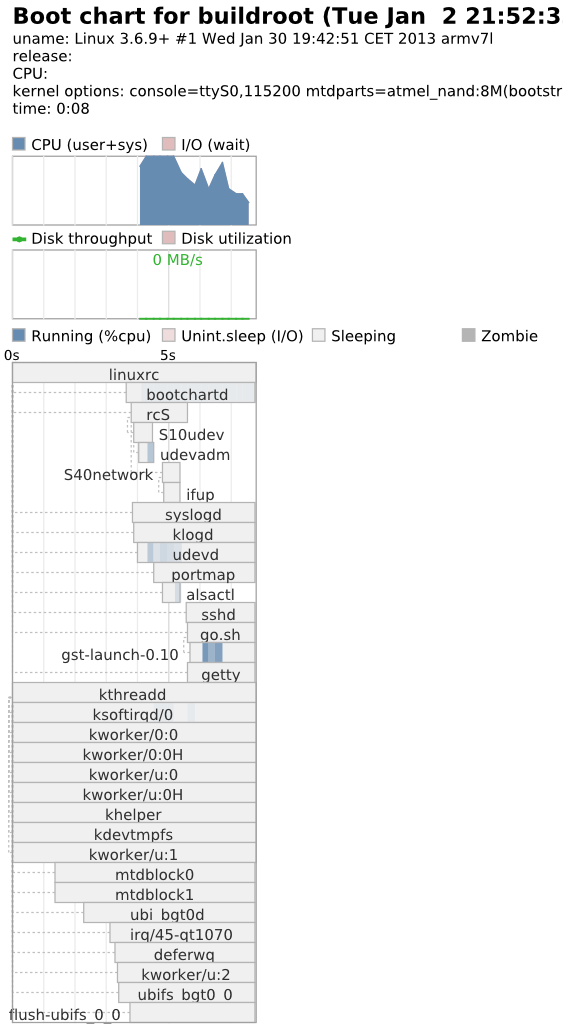
\includegraphics[height=0.8\textheight]{slides/boottime-init-scripts/bootchart.png}
\end{figure}
\end{frame}

\begin{frame}[fragile]
\frametitle{Measuring - bootchart}
\begin{itemize}
	\item You can use \code{bootchartd} from \code{busybox}
	      (\code{CONFIG_BOOTCHARTD=y})
	\item Boot your board passing \code{init=/sbin/bootchartd} on your
	      kernel command line
	\item Copy \code{/var/log/bootlog.tgz} from your target to your host
	\item Generate the timechart:
\begin{block}{}
\begin{verbatim}
cd bootchart-<version>
java -jar bootchart.jar bootlog.tgz
\end{verbatim}
\end{block}
\end{itemize}
\code{bootchart} is available at \url{http://www.bootchart.org}
\end{frame}

\begin{frame}[fragile]
\frametitle{Measuring - systemd}
If you are using \code{systemd} as your \code{init} program, you can use
\code{systemd-analyze}. See
\url{http://www.freedesktop.org/software/systemd/man/systemd-analyze.html}.\\
\begin{block}{}
\tiny
\begin{verbatim}
$ systemd-analyze blame
  6207ms udev-settle.service
   735ms NetworkManager.service
   642ms avahi-daemon.service
   600ms abrtd.service
   517ms rtkit-daemon.service
   396ms dbus.service
   390ms rpcidmapd.service
   346ms systemd-tmpfiles-setup.service
   316ms cups.service
   310ms console-kit-log-system-start.service
   309ms libvirtd.service
   303ms rpcbind.service
   298ms ksmtuned.service
   281ms rpcgssd.service
   277ms sshd.service
...
\end{verbatim}
\end{block}
\end{frame}

\begin{frame}
\frametitle{Initial measures}
In the initial demo, we measure the time taken to get the login
prompt (RomBOOT is excluded).
\begin{center}
    \includegraphics[width=\textwidth]{slides/boottime-init-scripts/timechart.pdf}
\end{center}
Total: 11.70s.
\end{frame}

\begin{frame}
\frametitle{Init}
Starting as soon as possible after all the dependencies are started:
\begin{itemize}
	\item Depends on your \code{init} program. Here we are assuming sysV
	      \code{init} scripts.
	\item \code{init} scripts run in alphanumeric order and start with
	      a letter (K for stop and S for start).
	\item You want to use the lowest number you can for your application.
	\item You can even replace \code{init} with your application!
\end{itemize}
How fast would we be if we could be the first started application?
\end{frame}

\begin{frame}
\frametitle{Results}
Before: 11.70s
\begin{center}
    \includegraphics[width=\textwidth]{slides/boottime-init-scripts/timechart.pdf}
\end{center}
After:
\begin{center}
    \includegraphics[width=\textwidth]{slides/boottime-init-scripts/timechart-init.pdf}
\end{center}
Total: 9.67s.
\end{frame}

\begin{frame}
\frametitle{Optimizing init scripts}
\begin{itemize}
	\item Start all your services directly from a single startup
	      script (e.g. \code{/etc/init.d/rcS}). This eliminates multiple
	      calls to \code{/bin/sh}.
	\item Replace \code{udev} with \code{mdev}. \code{mdev} is part of
	      BusyBox. It is not running as a daemon and you can either run it
   	      only once or have it handling hotplug events.
	\item Remove \code{udev} (or \code{mdev}) if you just need them
	      for device files.  Use \code{devtmpfs}
	      (\code{CONFIG_DEVTMPFS}) instead, automatically managed by the
	      kernel, and cheaper.
\end{itemize}
\end{frame}

\begin{frame}[fragile]
\frametitle{Reduce forking}
\begin{itemize}
	\item \code{fork}/\code{exec} system calls are very expensive.
		Because of this, calls to executables from shells are slow.
	\item Even executing \code{echo} in \code{busybox} shells results
	      in a \code{fork} syscall!
	\item Select \code{Shells -> Standalone shell} in \code{busybox}
	      configuration to make the \code{busybox} shell call applets
	      whenever possible.
	\item Pipes and back-quotes are also implemented by
	      \code{fork}/\code{exec}.  You can reduce their usage in
	      scripts. Example:
	      \begin{block}{}
			\begin{verbatim}
cat /proc/cpuinfo | grep model
			\end{verbatim}
		\end{block}
		Replace it with:
		\begin{block}{}
			\begin{verbatim}
grep model /proc/cpuinfo
			\end{verbatim}
		\end{block}
\end{itemize}
See \url{http://elinux.org/Optimize_RC_Scripts}
\end{frame}

\begin{frame}
\frametitle{Reduce size}
\begin{itemize}
	\item Strip your executables and libraries, removing ELF sections
		only needed for development and debugging. The \code{strip}
		command is provided by your cross-compiling toolchain.
		\code{BR2_STRIP_strip} in Buildroot.
	\item \code{superstrip}:
		\url{http://muppetlabs.com/~breadbox/software/elfkickers.html}.
		Goes beyond \code{strip} and can strip out a few more bits
		that are not used by Linux to start an executable.
		\code{BR2_STRIP_sstrip} in Buildroot.
	\item use \code{mklibs}, available at
		\url{http://packages.debian.org/sid/mklibs}.
		\code{mklibs} produces cut-down shared libraries that contain
		only the routines required by a particular set of executables.
		Really useful with big libraries like OpenGL and QT. It even
		works without having the source code but be careful as
		sometimes it can strip a bit too much (dlopened libraries).
\end{itemize}
\end{frame}

\setuplabframe
{Reducing time in init-scripts}
{
\begin{itemize}
\item Regenerate the root filesystem with Buildroot
\item Use bootchart to measure boot time
\end{itemize}
}


